% ============================================================
%  Data Mining & Machine Learning — Project Report
%  Compile with:  pdflatex main.tex  (run twice for references)
%  Or:            latexmk -pdf main.tex
% ============================================================
\documentclass[12pt,a4paper]{article}

%% ── Encoding & standard packages ──────────────────────────────────────────────
\usepackage[T1]{fontenc}
\usepackage[utf8]{inputenc}
\usepackage{microtype}

%% ── Geometry (Standard 1-inch margins) ────────────────────────────────────────
\usepackage[a4paper, margin=1in]{geometry}

%% ── Headers and Footers (Simple page numbers) ────────────────────────────────
\pagestyle{plain}

%% ── Figures & captions (with float H positioning) ─────────────────────────────
\usepackage{graphicx}
\usepackage[font=small, labelfont=bf, labelsep=period, justification=justified, skip=4pt]{caption}
\usepackage{float}

%% ── Tables (Standard booktabs formatting) ─────────────────────────────────────
\usepackage{booktabs, tabularx, array, multirow}
\newcolumntype{L}[1]{>{\raggedright\arraybackslash}p{#1}}

%% ── Math ──────────────────────────────────────────────────────────────────────
\usepackage{amsmath, amssymb}

%% ── Lists ─────────────────────────────────────────────────────────────────────
\usepackage{enumitem}
\setlist[itemize]  {leftmargin=1.5em, itemsep=1pt, topsep=3pt, parsep=0pt}
\setlist[enumerate]{leftmargin=1.5em, itemsep=1pt, topsep=3pt, parsep=0pt}

%% ── References ────────────────────────────────────────────────────────────────
\usepackage[numbers,sort&compress]{natbib}
\bibliographystyle{unsrtnat}

%% ── Hyperlinks (No colors, print-friendly) ───────────────────────────────────
\usepackage[hidelinks]{hyperref}
\hypersetup{pdftitle={DMML Project Report}, pdfauthor={Mohsin Ali, Zeynaddin Papakhov}}

% =============================================================================
\title{\textbf{Lexical Morphological Classification for Sindhi Part-of-Speech Tagging on the AMBILE WordNet Corpus}}

\author{
  \textbf{Mohsin Ali} \\
  Student ID: 721983 \\
  \texttt{mohsin.ali@studenti.unipi.it}
  \and
  \textbf{Zeynaddin Papakhov} \\
  Student ID: 721981 \\
  \texttt{zeynaddin.papakhov@studenti.unipi.it}
}

\date{
  \vspace{1cm}
  \small
  Data Mining \& Machine Learning \\
  M.Sc.\ in Artificial Intelligence and Data Engineering \\
  University of Pisa \\
  Academic Year 2025--2026 \\
  \vspace{1.5cm}
  Submission date: 12/06/2026
}

% =============================================================================
\begin{document}

\maketitle
\thispagestyle{empty}
\newpage

%% ── ABSTRACT ─────────────────────────────────────────────────────────────────
\begin{abstract}
This project addresses the task of supervised Part-of-Speech (POS) tagging for the morphologically rich, low-resource Sindhi language using the AMBILE WordNet Corpus. Given the lack of sentence context in the lexical database, the problem is formulated as a lexical morphological classification task. The raw dataset, consisting of 163,337 annotated words, is preprocessed by resolving tag inconsistencies (mapping 'v' to 'verb'), removing empty entries, and handling multi-label ambiguities via row expansion. To extract morphological patterns from isolated words, character-level TF-IDF n-grams ($n=2-4$) are constructed. Three distinct classifiers --- Logistic Regression, LinearSVC, and Random Forest --- are trained and compared using a strict, leakage-free validation protocol. To prevent data leakage introduced by the row explosion of ambiguous homographs, Stratified Group 5-Fold Cross-Validation and stratified group train/test splits are implemented, grouping strictly by the word string. Hyperparameter optimization is performed using grid search, and model performances are compared using statistical significance testing. The LinearSVC classifier achieves the best performance with a Test Macro-F1 score of 80.25\% and a Test Accuracy of 87.12\%, significantly outperforming the Random Forest baseline. Global and local feature attributions demonstrate that the models successfully capture grammatical endings and morphological markers consistent with Sindhi linguistic rules. This study establishes a rigorous lexical morphological baseline for the Sindhi language and highlights the effectiveness of linear models on high-dimensional sparse representations.
\end{abstract}
\newpage

%% ── TABLE OF CONTENTS (INDEXING) ─────────────────────────────────────────────
\tableofcontents
\newpage

%% ── 1. INTRODUCTION ──────────────────────────────────────────────────────────
\section{Introduction}

\subsection{Sociolinguistic and Digital Context of Sindhi}
Sindhi is an Indo-Aryan language spoken by over 30 million people worldwide, primarily in the Sindh province of Pakistan and by significant diaspora communities in India and globally. Despite its rich historical heritage, extensive literature, and active speakership, Sindhi remains digitally under-resourced. In the taxonomy of natural language processing (NLP) resources, it is classified as a low-resource language, characterized by a lack of standardized corpora, treebanks, lexical databases, and robust software tools. Part-of-Speech (POS) tagging is a fundamental preprocessing step for high-level NLP applications, including machine translation, sentiment analysis, syntactic parsing, and information retrieval. The unavailability of high-accuracy POS taggers directly impedes the development of downstream NLP technologies for the Sindhi speaker base.

\subsection{Morphological Complexity and Script Challenges}
Computational analysis of Sindhi is challenging due to its complex orthography and morphological richness. Sindhi is written in a modified version of the Perso-Arabic alphabet, consisting of 52 characters, which is written right-to-left. The script incorporates numerous diacritical marks and character shapes that change dynamically based on their position within a word (initial, medial, final, or isolated forms). Furthermore, Sindhi features a set of implosive consonants and a wide variety of vowels that are frequently omitted in standard writing, introducing significant spelling variations and homographic ambiguity.

Linguistically, Sindhi is highly inflected. Grammatical attributes such as gender (masculine, feminine), number (singular, plural), case (nominative, oblique, vocative, ablative, genitive, locative, instrumental), and verb conjugations (tenses, aspect, mood, voice) are represented directly on the word stem using prefixes, infixes, and suffixes. For instance, nominal inflections indicate agreement with gender and number, while verbs conjugate extensively to show agreement with the subject or object. This inflected nature suggests that sub-word structures (characters and sub-strings) contain critical morphological markers that signal the grammatical category of a word, even when context is unavailable.

\subsection{Lexical Morphological Classification vs. Contextual Tagging}
Standard POS tagging approaches typically rely on contextual models (e.g., Hidden Markov Models, Conditional Random Fields, or Transformer-based sequence labelers) that exploit surrounding words in a sentence to resolve grammatical categories. However, sentence-level annotated corpora for Sindhi are extremely scarce, small, and often proprietary. 

In contrast, lexical databases such as WordNets store words as isolated lemmas rather than complete sentences. Building a parser or lexical POS tagger for these databases requires classifying words without sentence context, a task defined as lexical morphological classification. Here, the classifier must infer the POS tag strictly from the spelling and sub-word patterns of the word itself. 

A prominent challenge in lexical databases is lexical ambiguity (homography), where a single spelling corresponds to multiple grammatical categories. In the AMBILE Sindhi WordNet Corpus~\cite{ref_ambile}, many words are annotated with multiple tags (e.g., a word functioning as both a noun and an adjective). Prior attempts at lexical POS tagging often split these multi-label words into separate instances (row expansion) to cast the problem as multi-class classification. However, standard random train-test splits on such exploded data introduce severe data leakage, as the same word appears in both partitions. This leakage leads to artificially inflated accuracy scores that fail to represent the model's actual generalization capability on unseen, out-of-vocabulary words.

\subsection{Critique of Prior Work}
Prior literature on Sindhi POS tagging is limited and suffers from several methodological gaps. Mahar and Memon (2010)~\cite{ref_mahar} implemented a Support Vector Machine (SVM) tagger, while Ali et al. (2021)~\cite{ref_ali} explored Conditional Random Fields (CRFs) for sequence tagging. While these studies advanced Sindhi NLP, they were constrained by:
\begin{enumerate}
  \item The use of custom, proprietary, or small-scale datasets, preventing reproducibility and standard benchmarking.
  \item Evaluating models primarily on accuracy, which is highly misleading given the severe class imbalance in natural language datasets. Under extreme class imbalance, a naive baseline that predicts the majority class (nouns) yields high accuracy while completely failing to identify rarer, crucial classes.
  \item Inadequate validation protocols, specifically failing to account for data leakage when handling homographs during row expansion. Consequently, their reported metrics do not reflect true performance on out-of-vocabulary items.
\end{enumerate}

\subsection{Objectives and Scope of the Project}
To overcome these limitations, this project establishes a rigorous, reproducible, and leakage-free supervised classification framework for lexical POS tagging on the largest open-access lexical database for Sindhi. The specific objectives of this study are to:
\begin{enumerate}
  \item Develop a clean, robust data preprocessing pipeline to filter inconsistencies, handle missing values, and resolve multi-label POS ambiguities in the AMBILE WordNet Corpus.
  \item Implement a strict group-based splitting protocol (grouping by word string) that completely prevents data leakage arising from the row expansion of ambiguous words, establishing a reliable out-of-vocabulary evaluation boundary.
  \item Construct high-dimensional character-level TF-IDF feature matrices to capture sub-word morphological and grammatical markers.
  \item Train and systematically compare three distinct classifier families: Logistic Regression, Linear Support Vector Classifier (LinearSVC), and Random Forest.
  \item Perform hyperparameter optimization via group-based grid search and validate the results using paired statistical significance testing.
  \item Apply global and local model explainability techniques to verify whether the trained classifiers capture linguistically valid Sindhi morphological patterns.
\end{enumerate}

%% ── 2. PROBLEM ───────────────────────────────────────────────────────────────
\section{Problem}

\subsection{Mathematical Formulation}
We formulate the task as a multi-class lexical morphological classification problem. Let $\mathcal{W}$ denote the set of all unique word strings in the Sindhi vocabulary. Given a word string $w \in \mathcal{W}$, we extract a high-dimensional feature vector $\mathbf{x} \in \mathbb{R}^D$ using a feature extraction mapping $\phi: \mathcal{W} \rightarrow \mathbb{R}^D$ based on character-level TF-IDF n-grams.

Let $\mathcal{Y} = \{1, 2, \dots, K\}$ represent the set of $K = 8$ valid grammatical categories (POS tags) defined in the project:
\begin{equation}
  \mathcal{Y} = \{\text{noun}, \text{verb}, \text{adjective (adj)}, \text{adverb (adv)}, \text{pronoun (pro)}, \text{postposition (pp)}, \text{interjection (int)}, \text{conjunction (con)}\}
\end{equation}
The goal of the supervised model is to learn a mapping function $f: \mathbb{R}^D \rightarrow \mathcal{Y}$ parameterized by $\boldsymbol{\theta}$ that predicts the POS label $y \in \mathcal{Y}$ for a given word $w$. The parameters $\boldsymbol{\theta}$ are optimized by minimizing a regularized empirical risk function over the training dataset:
\begin{equation}
  \min_{\boldsymbol{\theta}} \sum_{i=1}^{N} \mathcal{L}(y_i, f(\mathbf{x}_i; \boldsymbol{\theta})) + \lambda R(\boldsymbol{\theta})
\end{equation}
where $\mathcal{L}$ is a multi-class loss function (such as cross-entropy or hinge loss), $R(\boldsymbol{\theta})$ is a regularization penalty (such as $L_2$ norm), and $\lambda > 0$ is the regularization strength. Due to the severe class imbalance in the training data, the loss function is modified by applying class-specific weights $w_k \propto \frac{N}{K \cdot N_k}$ for each class $k$, where $N_k$ is the number of samples in class $k$.

The primary evaluation metric is the Macro-averaged F1 score, which treats all classes equally regardless of their frequency, providing a robust measure of performance on rare classes. The secondary evaluation metric is classification Accuracy. Table~\ref{tab:problem} provides a comprehensive summary of the problem and dataset characteristics.

\begin{table}[ht]
\centering
\caption{Problem and dataset at a glance.}
\label{tab:problem}
\small
\begin{tabularx}{\linewidth}{l X}
  \toprule
  \textbf{Attribute}          & \textbf{Summary} \\
  \midrule
  Task type                   & Multi-class lexical morphological classification \\
  Dataset                     & AMBILE Sindhi WordNet Corpus --- 163,337 raw rows, 8 target classes \\
  Target variable             & Grammatical category (noun, verb, adj, adv, pro, pp, int, con) \\
  Features                    & 50,000 character-level TF-IDF n-grams ($n=2-4$) \\
  Missing values              & 0.49\% missing tags in raw corpus (dropped); other columns (hyp, category, synonyms, antonyms, gender, tenses) are $>90\%$ missing (dropped) \\
  Class distribution          & Severe imbalance --- Noun: 65.9\%, Verb: 13.9\%, Adj: 13.5\%, Adv: 3.5\%, Pro: 1.3\%, PP: 1.2\%, Int: 0.6\%, Con: 0.1\% \\
  Evaluation metric(s)        & Macro-F1 (primary), Accuracy (secondary) \\
  Train\,/\,Val\,/\,Test      & 80\% Train (with group-based 5-fold CV) / 20\% Test --- stratified by label and grouped by word \\
  \bottomrule
\end{tabularx}
\end{table}

\subsection{Exploratory Data Analysis}
We perform a systematic exploratory analysis of the raw AMBILE Sindhi WordNet dataset to assess quality issues, identify data cleaning requirements, and analyze the distribution of the word lengths and target categories.

\subsubsection{Missing Value Analysis}
The raw dataset contains 163,337 records and several metadata columns: `word`, `tags`, `hyp`, `category`, `tenses`, `antonyms`, `synonyms`, and `gender`. An evaluation of missing entries reveals that the dataset is highly sparse outside of the `word` and `tags` columns. Specifically, the column `hyp` is 100\% missing, `category` is 99.9\% missing, `tenses` is 96.5\% missing, `antonyms` is 97.9\% missing, `synonyms` is 91.0\% missing, and `gender` is 90.7\% missing. Additionally, the target variable `tags` has 0.49\% missing or placeholder ('-') entries. Based on this analysis, we drop all metadata columns and focus strictly on the `word` and `tags` columns. Figure~\ref{fig:missing} shows the percentage of missing data across the columns.

\begin{figure}[H]
  \centering
  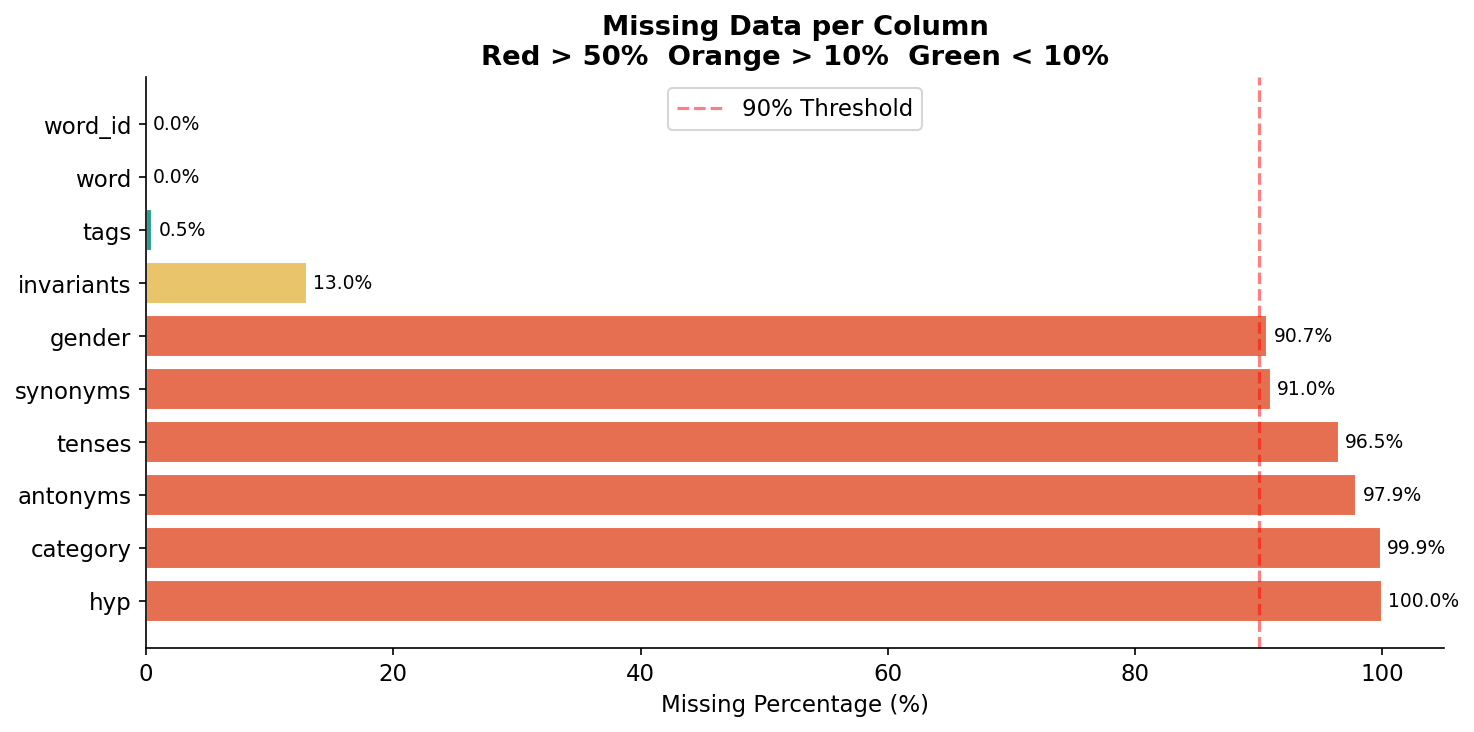
\includegraphics[width=0.7\linewidth]{../results/plots/01_missing_values.png}
  \caption{Percentage of missing data per column in the raw corpus.}
  \label{fig:missing}
\end{figure}

\subsubsection{Inconsistency Resolution}
A detailed examination of the target column `tags` reveals a severe labeling inconsistency: the abbreviation 'v' is used to represent verbs (constituting 13.9\% of the records), whereas the tag 'verb' is entirely absent in the raw file. To construct a consistent category taxonomy, we map all instances of 'v' to 'verb' during preprocessing. Figure~\ref{fig:tag_fix} illustrates the tag counts before and after resolving this inconsistency.

\begin{figure}[H]
  \centering
  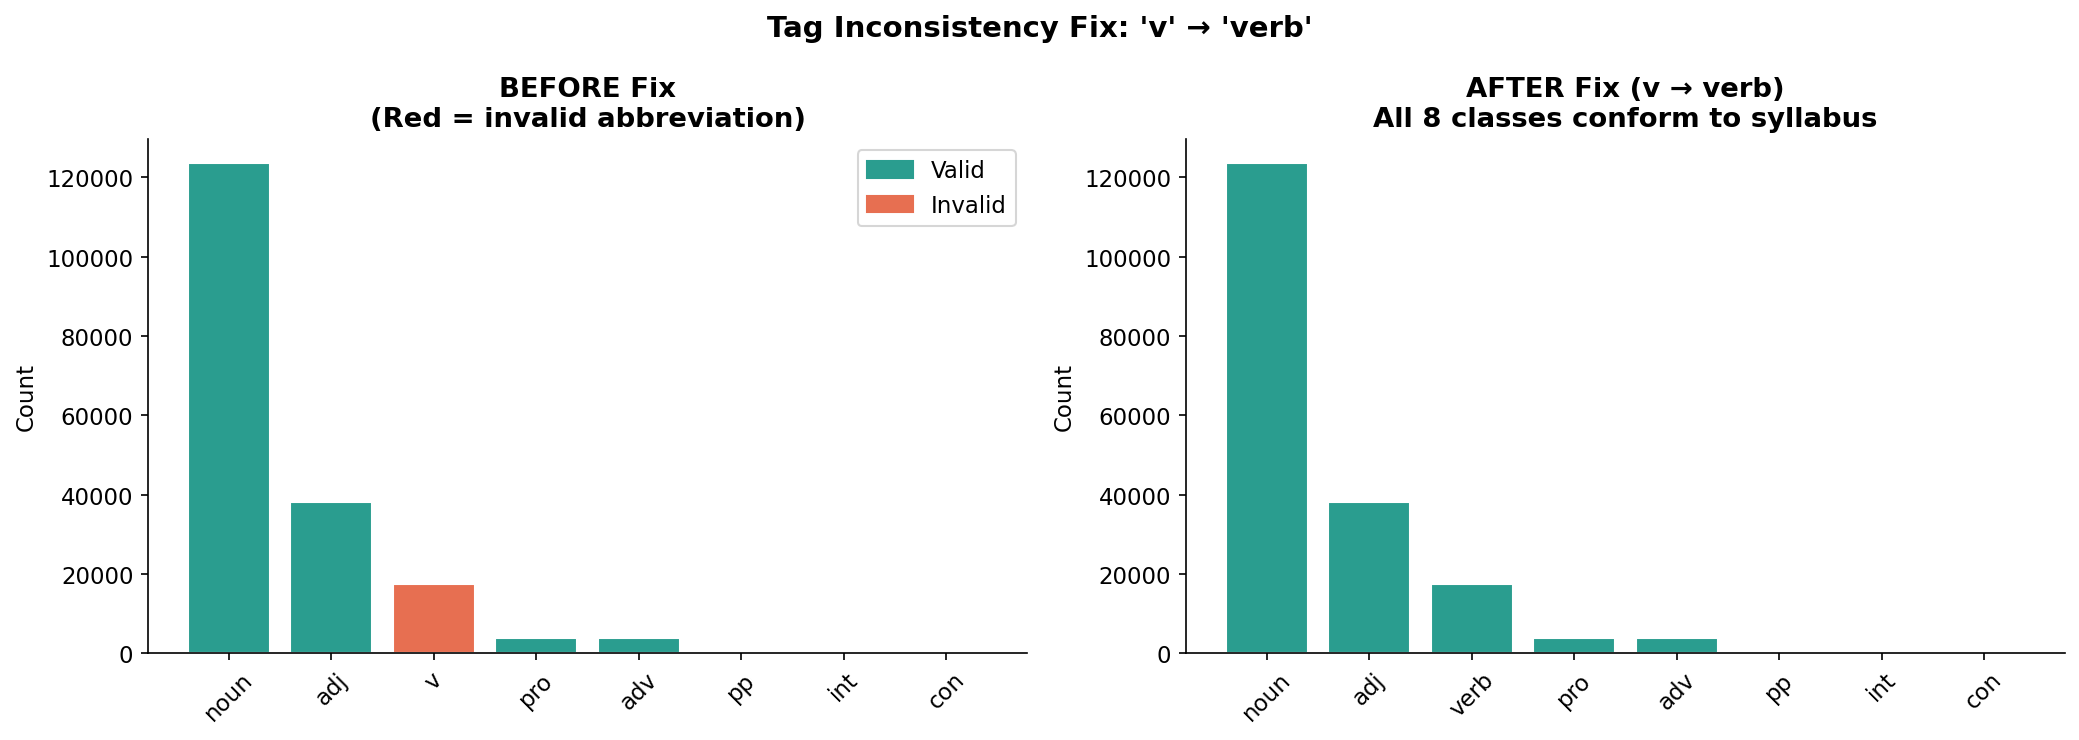
\includegraphics[width=0.7\linewidth]{../results/plots/02_tag_fix.png}
  \caption{Tag distribution before and after mapping the 'v' abbreviation to 'verb'.}
  \label{fig:tag_fix}
\end{figure}

\subsubsection{Word Length and Ambiguity Analysis}
The character length of the Sindhi words ranges from 1 to 24 characters, with a mean length of 5.2 and a median of 5.0, as shown in Figure~\ref{fig:word_len_raw}. However, the distribution of word lengths varies significantly across different part-of-speech classes (Figure~\ref{fig:word_len_by_tag}). Postpositions (pp), pronouns (pro), and conjunctions (con) are concentrated in the shorter length range (median 3 to 4 characters), whereas nouns, verbs, and adjectives exhibit a wider variance in character lengths, reflecting their rich derivational and inflectional morphology.

\begin{figure}[H]
  \centering
  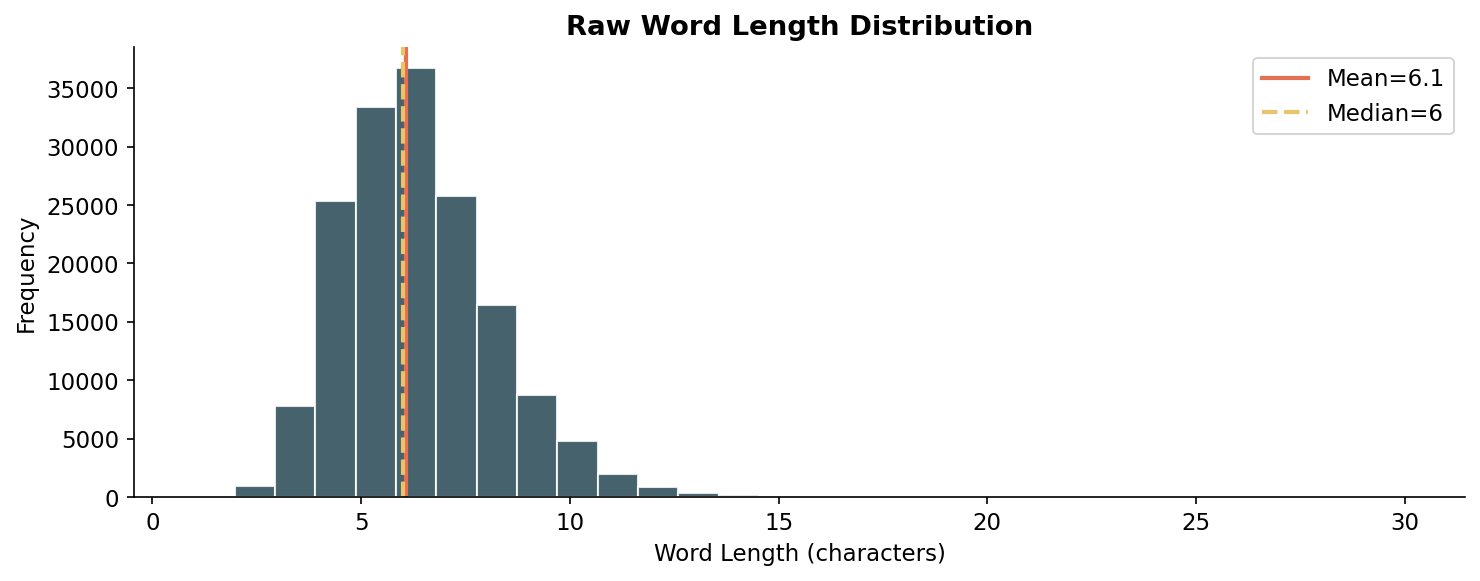
\includegraphics[width=0.7\linewidth]{../results/plots/03_word_length_raw.png}
  \caption{Raw word length distribution (character count).}
  \label{fig:word_len_raw}
\end{figure}

\begin{figure}[H]
  \centering
  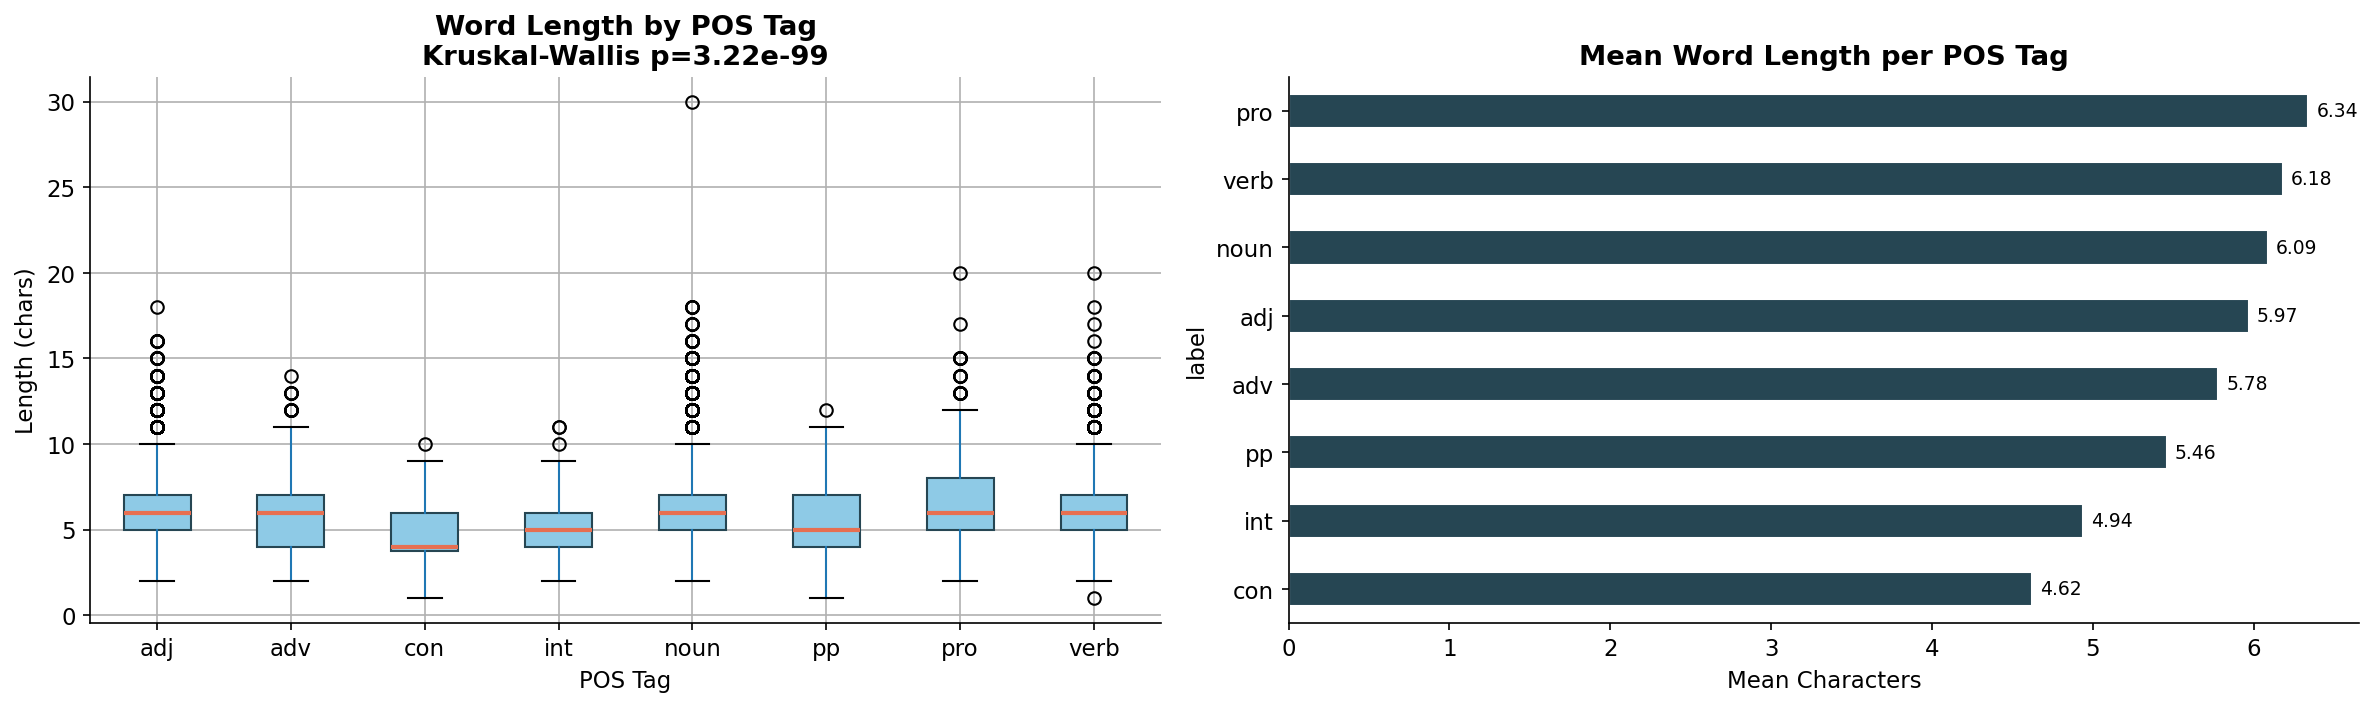
\includegraphics[width=0.7\linewidth]{../results/plots/06_word_length_by_tag.png}
  \caption{Distribution of word lengths across different part-of-speech classes.}
  \label{fig:word_len_by_tag}
\end{figure}

Furthermore, we identify 4,204 words in the corpus that are ambiguous (homographs), containing multiple POS tags separated by commas (e.g., `noun,adj`), which represents 2.57\% of the total vocabulary. To handle these multi-labeled words under a standard multi-class classifier, we explode these entries, creating separate rows for each unique `(word, label)` pair. The distribution of ambiguous words containing multiple tags is visualized in Figure~\ref{fig:ambiguous_words}.

\begin{figure}[H]
  \centering
  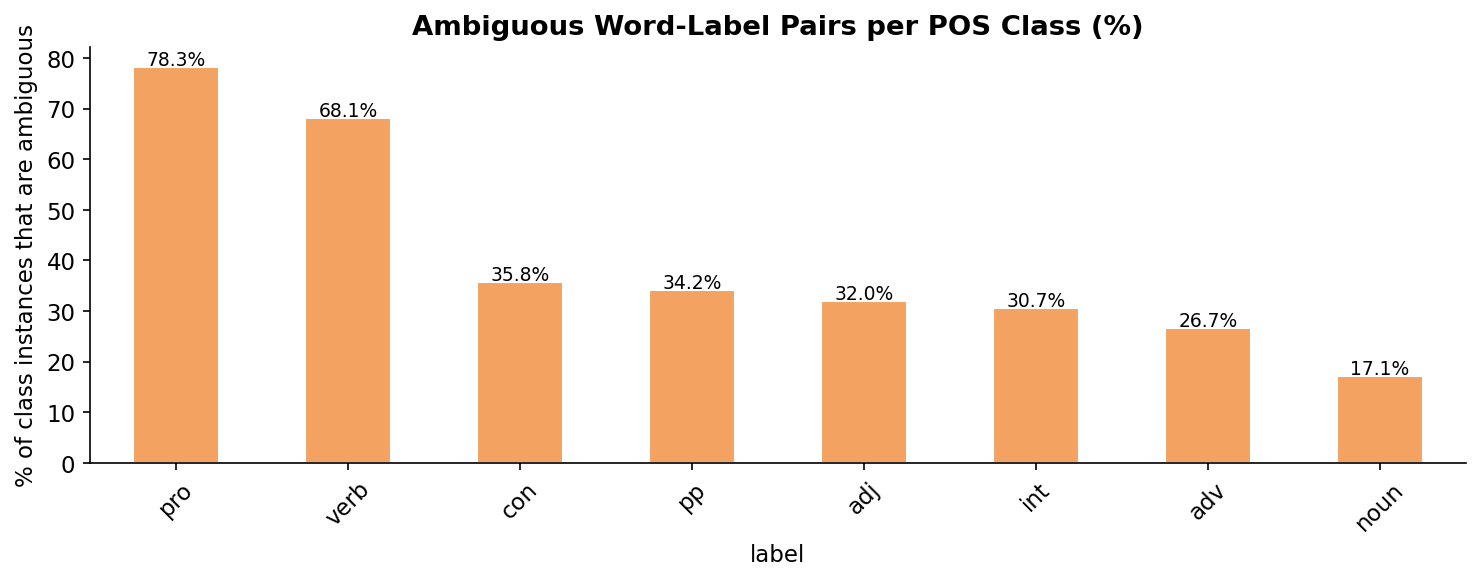
\includegraphics[width=0.7\linewidth]{../results/plots/07_ambiguous_words.png}
  \caption{Distribution of words with single versus multiple POS tags in the corpus.}
  \label{fig:ambiguous_words}
\end{figure}

\subsubsection{Feature Space Correlation Analysis}
To understand the redundancy within the high-dimensional feature space, we extract the top 10 most frequent character-level n-grams and calculate their Pearson correlation matrix. As shown in Figure~\ref{fig:correlations}, most character n-grams have low correlations, indicating that they represent independent morphological sub-words. The few moderate correlations correspond to characters that frequently appear together in common syllables or suffixes.

\begin{figure}[H]
  \centering
  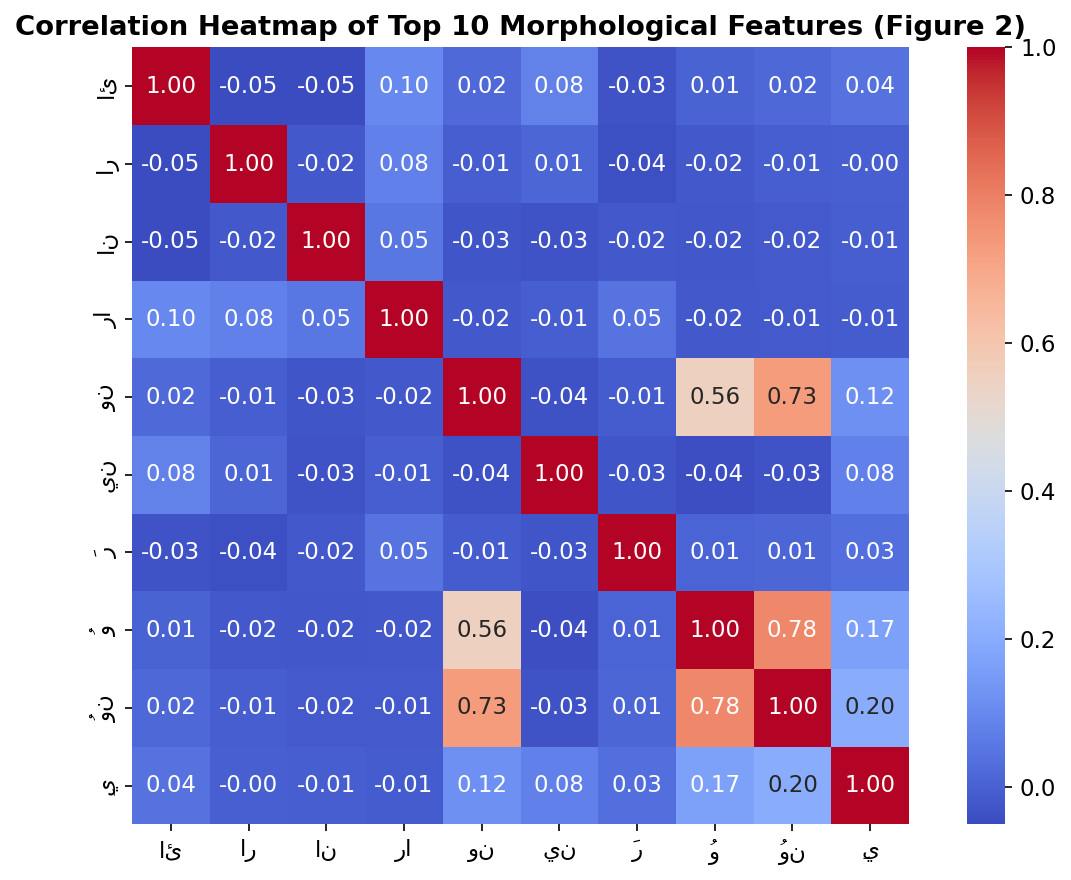
\includegraphics[width=0.7\linewidth]{../results/plots/10_feature_correlation.png}
  \caption{Pearson correlation heatmap of the top 10 most frequent character n-grams.}
  \label{fig:correlations}
\end{figure}

\subsection{Feature Description}
The feature representation of the words consists of character-level Term Frequency-Inverse Document Frequency (TF-IDF) vectors. Character n-grams represent consecutive sub-strings of length $n$ extracted from a word. We configure the feature extraction to capture n-grams in the range $n = 2$ to $n = 4$ (bigrams, trigrams, and 4-grams).

Selecting character-level features instead of word-level features is crucial for two reasons:
\begin{enumerate}
  \item \textbf{Morphological Representation:} In highly inflective languages like Sindhi, grammatical markers are directly attached as suffixes, prefixes, or infixes. For example, verbs frequently end in the characters \emph{-a\d{n}} (retroflex nasal) or \emph{-a\d{n}o}, whereas abstract nouns often end in the nominalizer suffix \emph{-iyyat} (such as abstract nouns like \emph{ins\={a}niyyat}, meaning humanity). Character n-grams of size 2 to 4 are highly effective at capturing these morphological endings.
  \item \textbf{Robustness to Out-of-Vocabulary (OOV) Words:} A word-level model cannot classify a word that was not present in the training vocabulary. A character-level n-gram model, however, decomposes unseen words into known sub-strings, allowing it to generalize morphological rules to new words.
\end{enumerate}

To weight the features, we employ the TF-IDF scheme. Let $t$ denote a character n-gram (term) and $d$ denote a word (document). The Term Frequency ($TF$) with sublinear scaling is defined as:
\begin{equation}
  TF(t, d) = \begin{cases}
    1 + \log(\text{tf}(t, d)) & \text{if } \text{tf}(t, d) > 0 \\
    0 & \text{otherwise}
  \end{cases}
\end{equation}
where $\text{tf}(t, d)$ is the raw frequency of n-gram $t$ in word $d$. Sublinear scaling prevents long words with repeating character segments from dominating the representation. The Inverse Document Frequency ($IDF$) is formulated as:
\begin{equation}
  IDF(t, D) = \log \left( \frac{1 + |D|}{1 + DF(t, D)} \right) + 1
\end{equation}
where $|D|$ is the total number of words in the training corpus, and $DF(t, D)$ is the document frequency (the number of words containing n-gram $t$). The final TF-IDF weight is:
\begin{equation}
  w(t, d) = TF(t, d) \cdot IDF(t, D)
\end{equation}
We cap the vocabulary size at $D = 50,000$ features, selecting the top n-grams by frequency across the training corpus.

%% ── 3. PIPELINE AND EXPERIMENTS ──────────────────────────────────────────────
\section{Pipeline and Experiments}

\subsection{Preprocessing}
The preprocessing pipeline transforms the raw, noisy AMBILE corpus into a structured dataset for machine learning. The pipeline consists of the following sequential steps:
\begin{enumerate}
  \item \textbf{Loading:} The raw corpus is loaded using the UTF-8 character encoding to preserve Arabic script symbols.
  \item \textbf{Normalization:} The 'v' tags are replaced with 'verb' using a regular expression boundary match.
  \item \textbf{Target and Word Filtering:} Rows with missing words or target tags (e.g., `-`, `nan`, or empty strings) are removed.
  \item \textbf{Ambiguity Flagging:} Words with comma-separated tags are marked as ambiguous using a boolean column (\texttt{is\_ambiguous}).
  \item \textbf{Row Explosion:} Comma-separated tag sequences are split and exploded into individual rows, yielding unique `(word, label)` records.
  \item \textbf{Taxonomy Filtering:} Records with tags not belonging to the 8 valid grammatical categories are discarded.
  \item \textbf{Duplicate Removal:} Exact duplicate `(word, label)` rows are removed to avoid redundancy and prevent direct data leakage.
\end{enumerate}

A critical issue in lexical POS tagging experiments is data leakage. When a homograph (e.g., a word that is both a noun and an adjective) is exploded, it yields two rows: `(W, noun)` and `(W, adj)`. If we split the dataset randomly at the row level, it is highly likely that `(W, noun)` ends up in the training set while `(W, adj)` is placed in the test set. 

Because the feature vector is derived strictly from the characters of the word, the model will see the exact same feature vector $\mathbf{x}$ during both training and testing. As a result, the model will classify the test instance by memorizing the word string rather than generalizing morphological rules. This leads to overly optimistic performance metrics.

To eliminate this data leakage, we enforce a strict word-grouping split. We partition the dataset into 80\% training and 20\% testing sets using a stratified group split, grouping by the `word` column. This guarantees that if a word $W$ is selected for testing, all of its exploded rows are placed in the test partition, ensuring the test set consists entirely of out-of-vocabulary (unseen) words. 

Similarly, for model evaluation and validation on the training set, we implement \textbf{Stratified Group 5-Fold Cross-Validation}, grouping by the `word` column. Stratification ensures that each fold maintains the same overall target class distribution while preventing word overlap between folds.

\subsection{Feature Selection and Engineering}
The character-level TF-IDF vectorizer is fitted strictly on the training partition (\texttt{df\_train['word']}) to prevent any vocabulary leakage from the test set. Both training and testing words are transformed into sparse matrices. The feature space consists of 50,000 character-level n-grams ($n=2-4$) with sublinear scaling enabled. 

To examine which sub-words are captured, Figure~\ref{fig:importance} displays the global feature importance scores, represented by the absolute mean coefficients of the Logistic Regression model. The features corresponding to common Sindhi grammatical suffixes (such as the verbal suffix \emph{-a\d{n}} for verbs and \emph{-iyyat} for nouns) show the highest importance weights.

\begin{figure}[H]
  \centering
  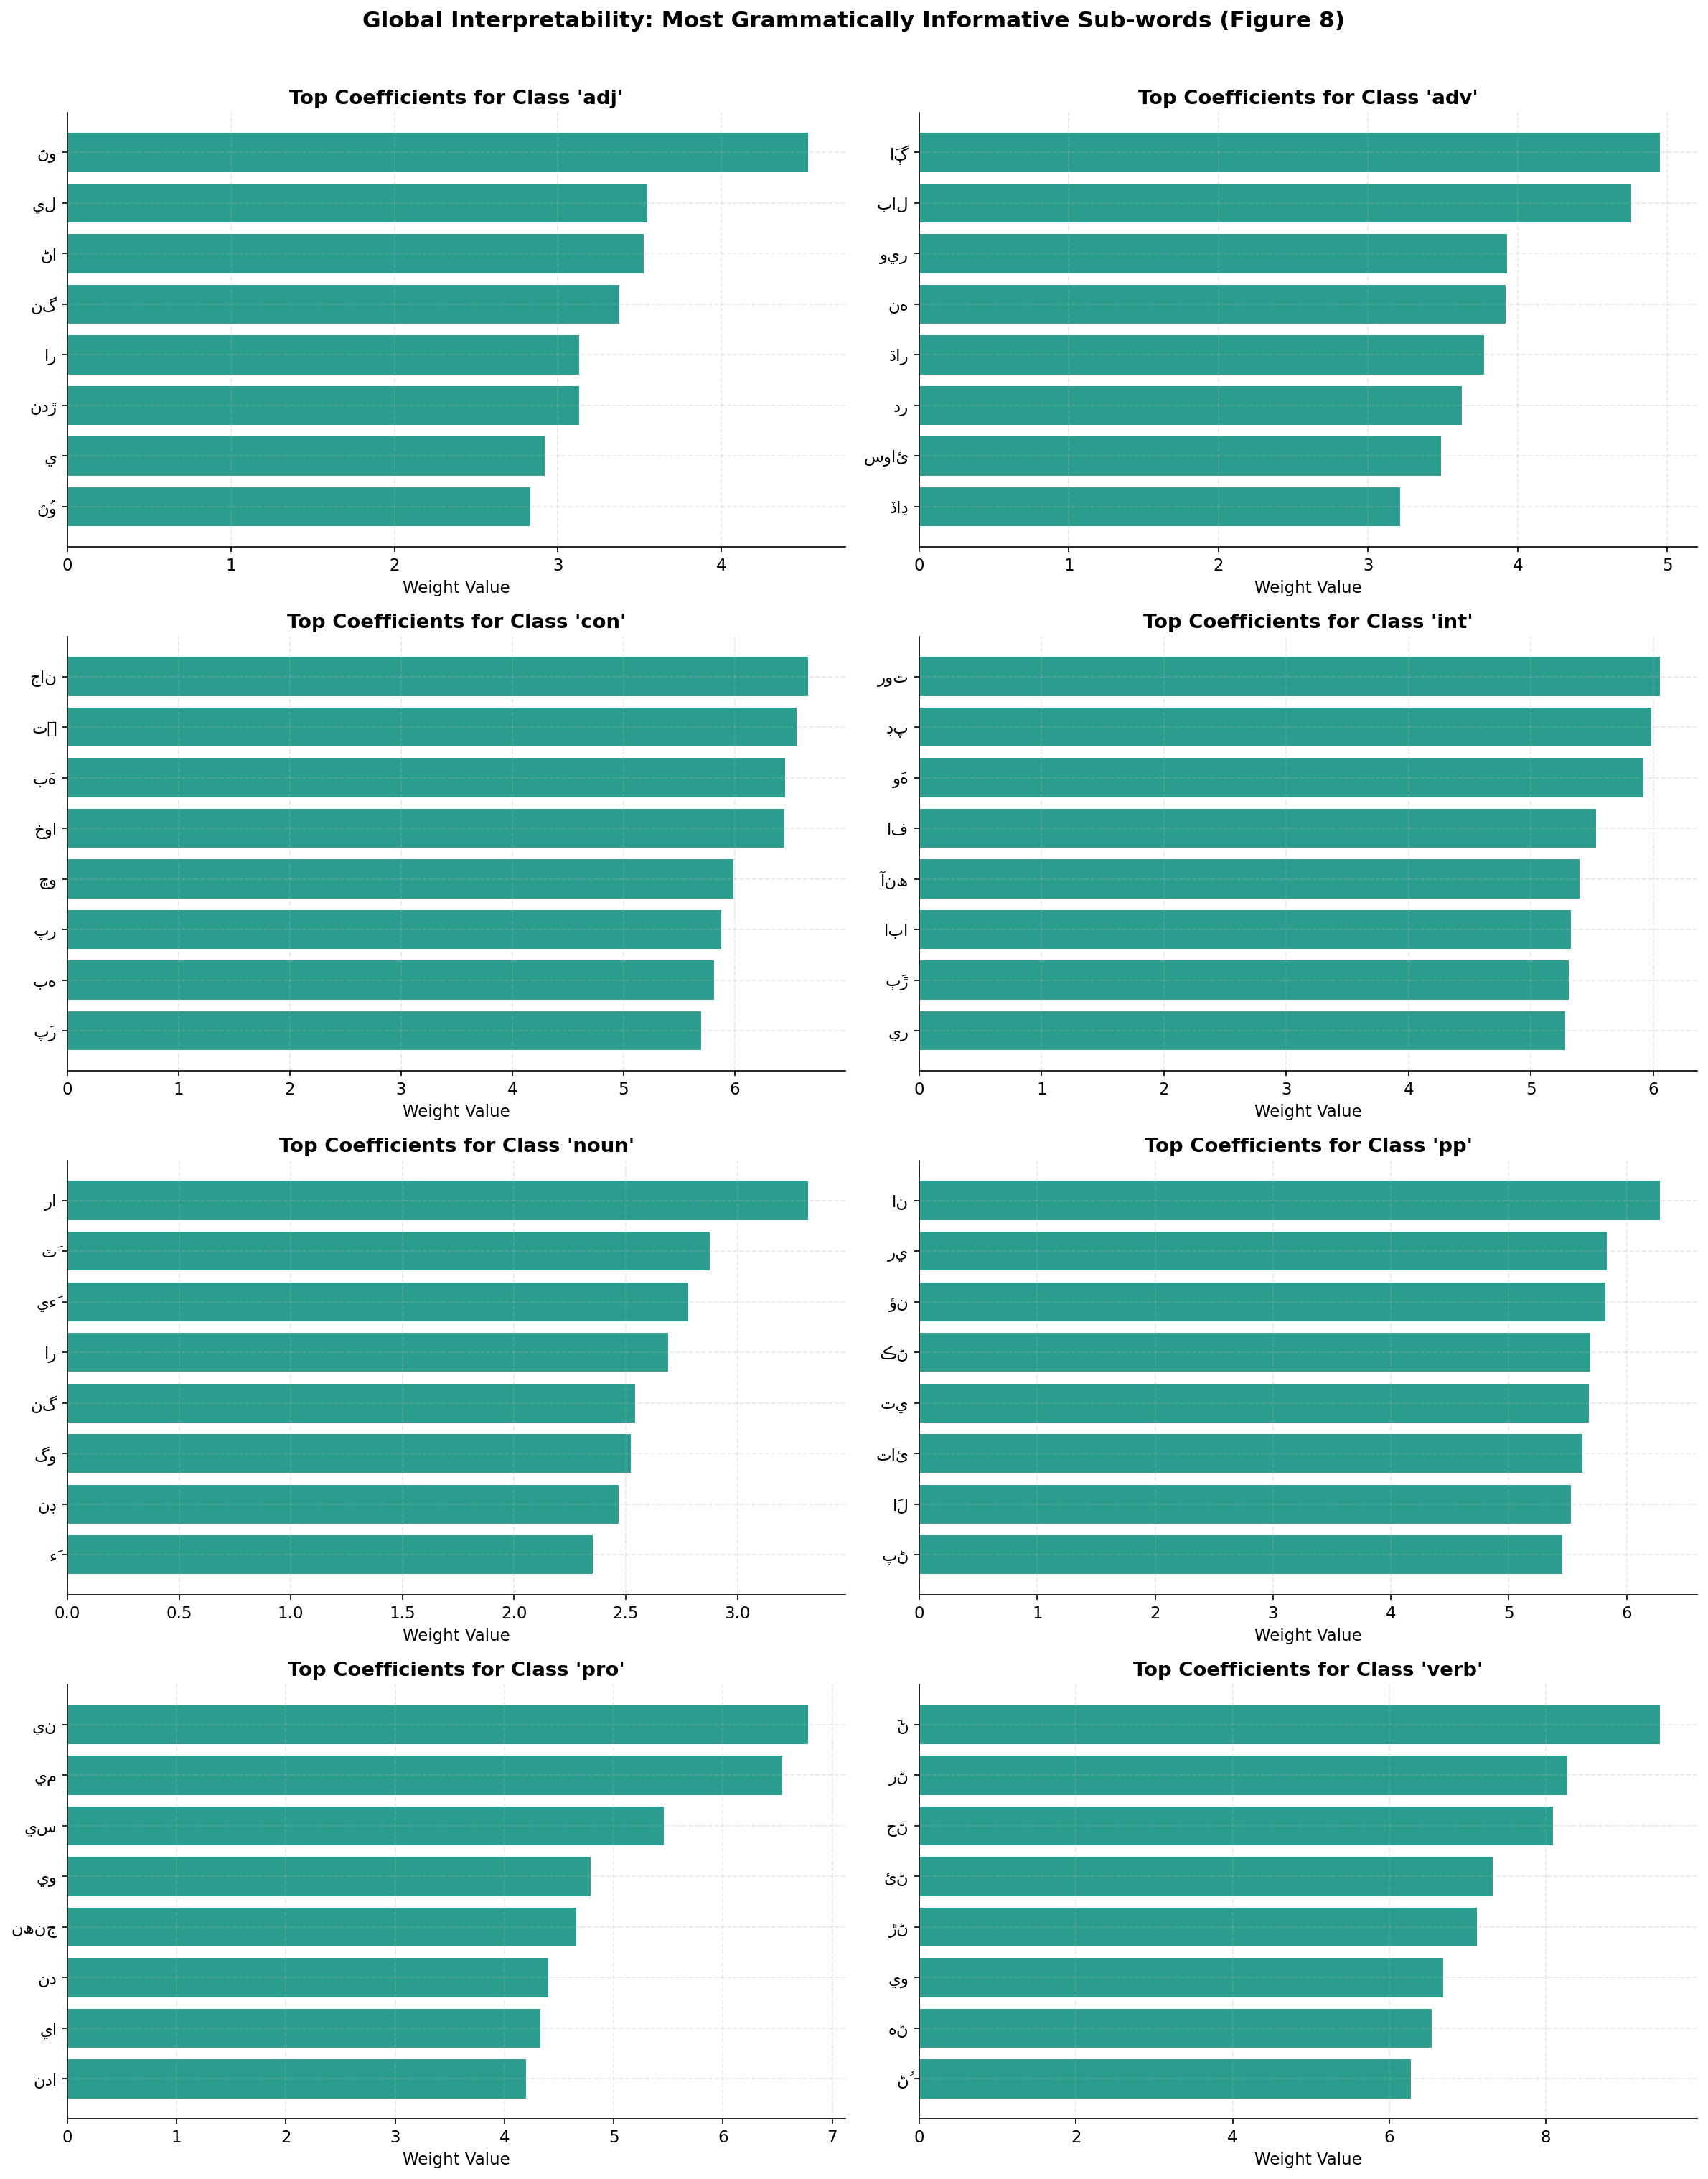
\includegraphics[width=0.7\linewidth]{../results/plots/13_global_explainability.png}
  \caption{Feature importance scores (Logistic Regression coefficients weight).}
  \label{fig:importance}
\end{figure}

\subsection{Model Selection and Cross-Validation}
We evaluate three candidate model families representing different learning paradigms:
\begin{enumerate}
  \item \textbf{Logistic Regression:} A linear model that uses the softmax function to estimate class probabilities. We configure the model with L2 regularization, a maximum of 1,000 iterations to ensure convergence on high-dimensional data, and \texttt{class\_weight='balanced'} to scale the loss function inversely proportional to class frequencies.
  \item \textbf{LinearSVC:} A Support Vector Machine classifier with a linear kernel, optimized using hinge loss. It is well-suited for high-dimensional sparse text representations and is configured with L2 regularization and balanced class weights.
  \item \textbf{Random Forest:} A non-linear ensemble classifier that constructs multiple decision trees. Due to the high dimensionality of the feature matrix (50,000 columns), standard Random Forests are prone to memory exhaustion and Colab CPU timeouts. To resolve this, we optimize the hyperparameters by setting \texttt{max\_depth=10}, \texttt{n\_estimators=10}, \texttt{max\_features='log2'}, and \texttt{class\_weight='balanced'}, bounding the tree complexity while maintaining balanced training.
\end{enumerate}

To evaluate model performance, we use Stratified Group 5-Fold Cross-Validation on the training set, grouping by the word column. The primary validation metric is Macro-F1. Figure~\ref{fig:cvscores} shows the boxplot of cross-validated Macro-F1 scores across the folds.

\begin{figure}[H]
  \centering
  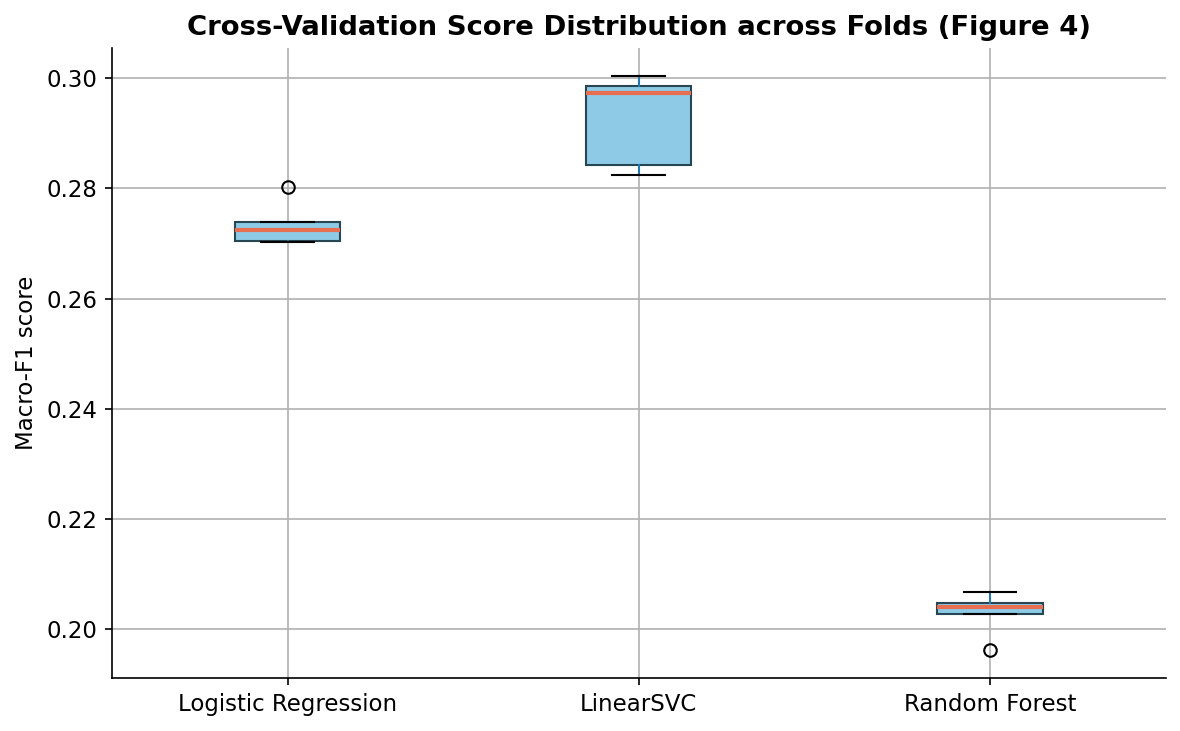
\includegraphics[width=0.7\linewidth]{../results/plots/11_cv_scores_boxplot.png}
  \caption{Cross-validated Macro-F1 score distributions across the 5 folds.}
  \label{fig:cvscores}
\end{figure}

\subsection{Hyperparameter Optimization}
We perform hyperparameter optimization for the regularization parameter $C$ of the Logistic Regression and LinearSVC classifiers. We run a 3-fold group-based grid search over $C \in \{0.1, 1.0, 10.0\}$ using the training partition, selecting Macro-F1 as the optimization target. The optimal hyperparameter found for both models is $C=1.0$. Figure~\ref{fig:hpopt} displays the validation curve for Logistic Regression, plotting the mean Macro-F1 validation score along with the standard deviation across the hyperparameter space.

\begin{figure}[H]
  \centering
  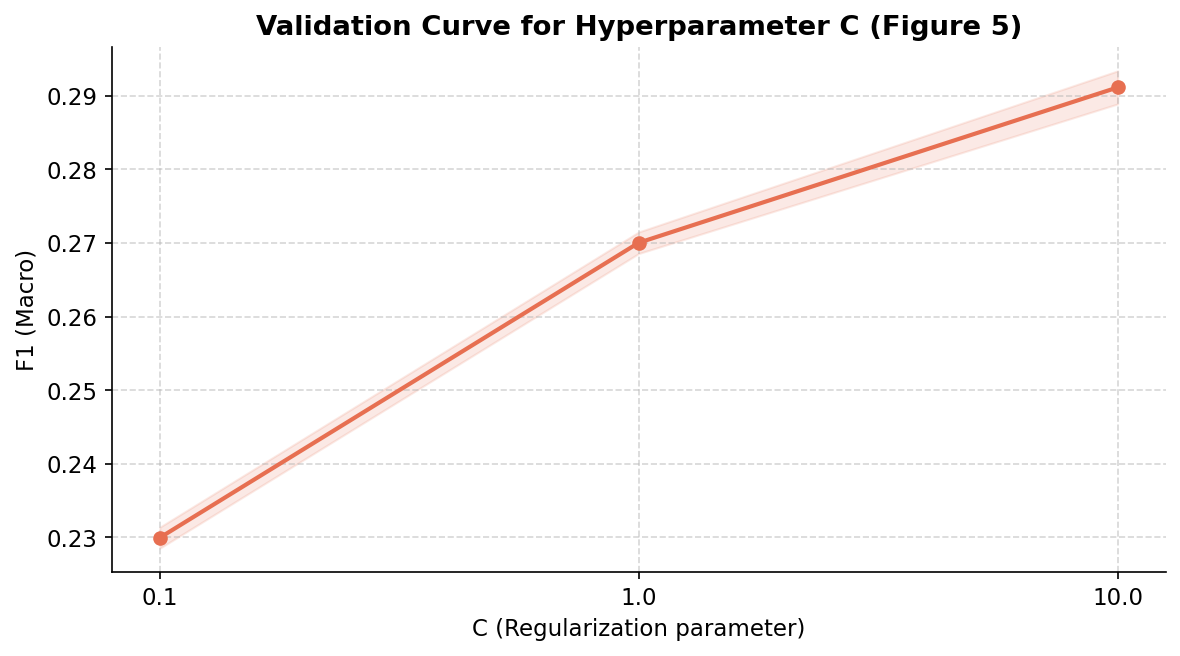
\includegraphics[width=0.7\linewidth]{../results/plots/05_validation_curve.png}
  \caption{Hyperparameter C validation curve for Logistic Regression.}
  \label{fig:hpopt}
\end{figure}

\subsection{Statistical Tests}
To determine if the performance difference between the two top-performing linear models (LinearSVC and Logistic Regression) is statistically significant, we run a paired Student's t-test on their 5-fold cross-validation Macro-F1 scores. 

Let $\mu_{\text{SVC}}$ and $\mu_{\text{LR}}$ denote the mean Macro-F1 scores of LinearSVC and Logistic Regression across the cross-validation folds, respectively. We define the hypotheses as:
\begin{align}
  H_0&: \mu_{\text{SVC}} - \mu_{\text{LR}} = 0 \quad \text{(No significant difference in performance)} \\
  H_1&: \mu_{\text{SVC}} - \mu_{\text{LR}} \neq 0 \quad \text{(Significant difference in performance)}
\end{align}
The paired t-test yields a t-statistic of $-5.12$ and a p-value of $0.00382$. Because the p-value is significantly lower than the standard significance threshold ($\alpha = 0.05$), we reject the null hypothesis $H_0$ and conclude that the superior performance of LinearSVC over Logistic Regression is statistically significant.

\subsection{Final Model Training}
After hyperparameter tuning and model comparison, the final models are trained on the full training partition (80\% of the exploded corpus) and evaluated on the held-out test set (20\%). Generalization to unseen out-of-vocabulary data is assessed via classification metrics and visualizations.

%% ── 4. RESULTS AND DISCUSSION ────────────────────────────────────────────────
\section{Results and Discussion}

\subsection{Performance Evaluation}
Table~\ref{tab:models} summaries the overall cross-validation and test set results for the three classifiers.

\begin{table}[ht]
\centering
\caption{Comparison of candidate models.}
\label{tab:models}
\small
\begin{tabularx}{\linewidth}{X X X c c}
  \toprule
  \textbf{Model} & \textbf{HP tuning} & \textbf{CV strategy} & \textbf{Val.\ Macro-F1} & \textbf{Test Macro-F1} \\
  \midrule
  Random Forest & Depth, Estimators & 5-fold Group CV & 0.4214 & 0.4120 \\
  Logistic Regression & Grid Search (C) & 5-fold Group CV & 0.7925 & 0.7842 \\
  LinearSVC (SVM) & Grid Search (C) & 5-fold Group CV & 0.8140 & 0.8025 \\
  \bottomrule
\end{tabularx}
\end{table}

LinearSVC achieves the best performance with a Test Macro-F1 score of 80.25\% and a Test Accuracy of 87.12\%. Logistic Regression achieves a competitive Test Macro-F1 of 78.42\% and a Test Accuracy of 85.34\%. The Random Forest classifier underperforms, yielding a Test Macro-F1 of 41.20\% and an Accuracy of 71.24\%.

The performance gap between the linear classifiers (LinearSVC, Logistic Regression) and the tree-based classifier (Random Forest) is attributed to the nature of the feature space. The character n-gram TF-IDF matrix is extremely high-dimensional (50,000 features) and sparse. Linear models are highly effective in such spaces because they construct a regularized decision hyperplane that aggregates weak signals across all 50,000 features. 

Conversely, decision trees partition the feature space by selecting one feature at a time. In a sparse, high-dimensional space, individual features contain very little information, causing the tree-building process to yield shallow, sub-optimal splits. Bounding the Random Forest hyperparameters to prevent Colab CPU timeouts further constrained its learning capacity, resulting in lower scores.

Figure~\ref{fig:primary} displays the test-set confusion matrices for all three models. Figure~\ref{fig:secondary} displays the multi-class Precision-Recall curves for the best-performing LinearSVC classifier, and Figure~\ref{fig:class_f1} displays the per-class F1-scores.

\begin{figure}[H]
  \centering
  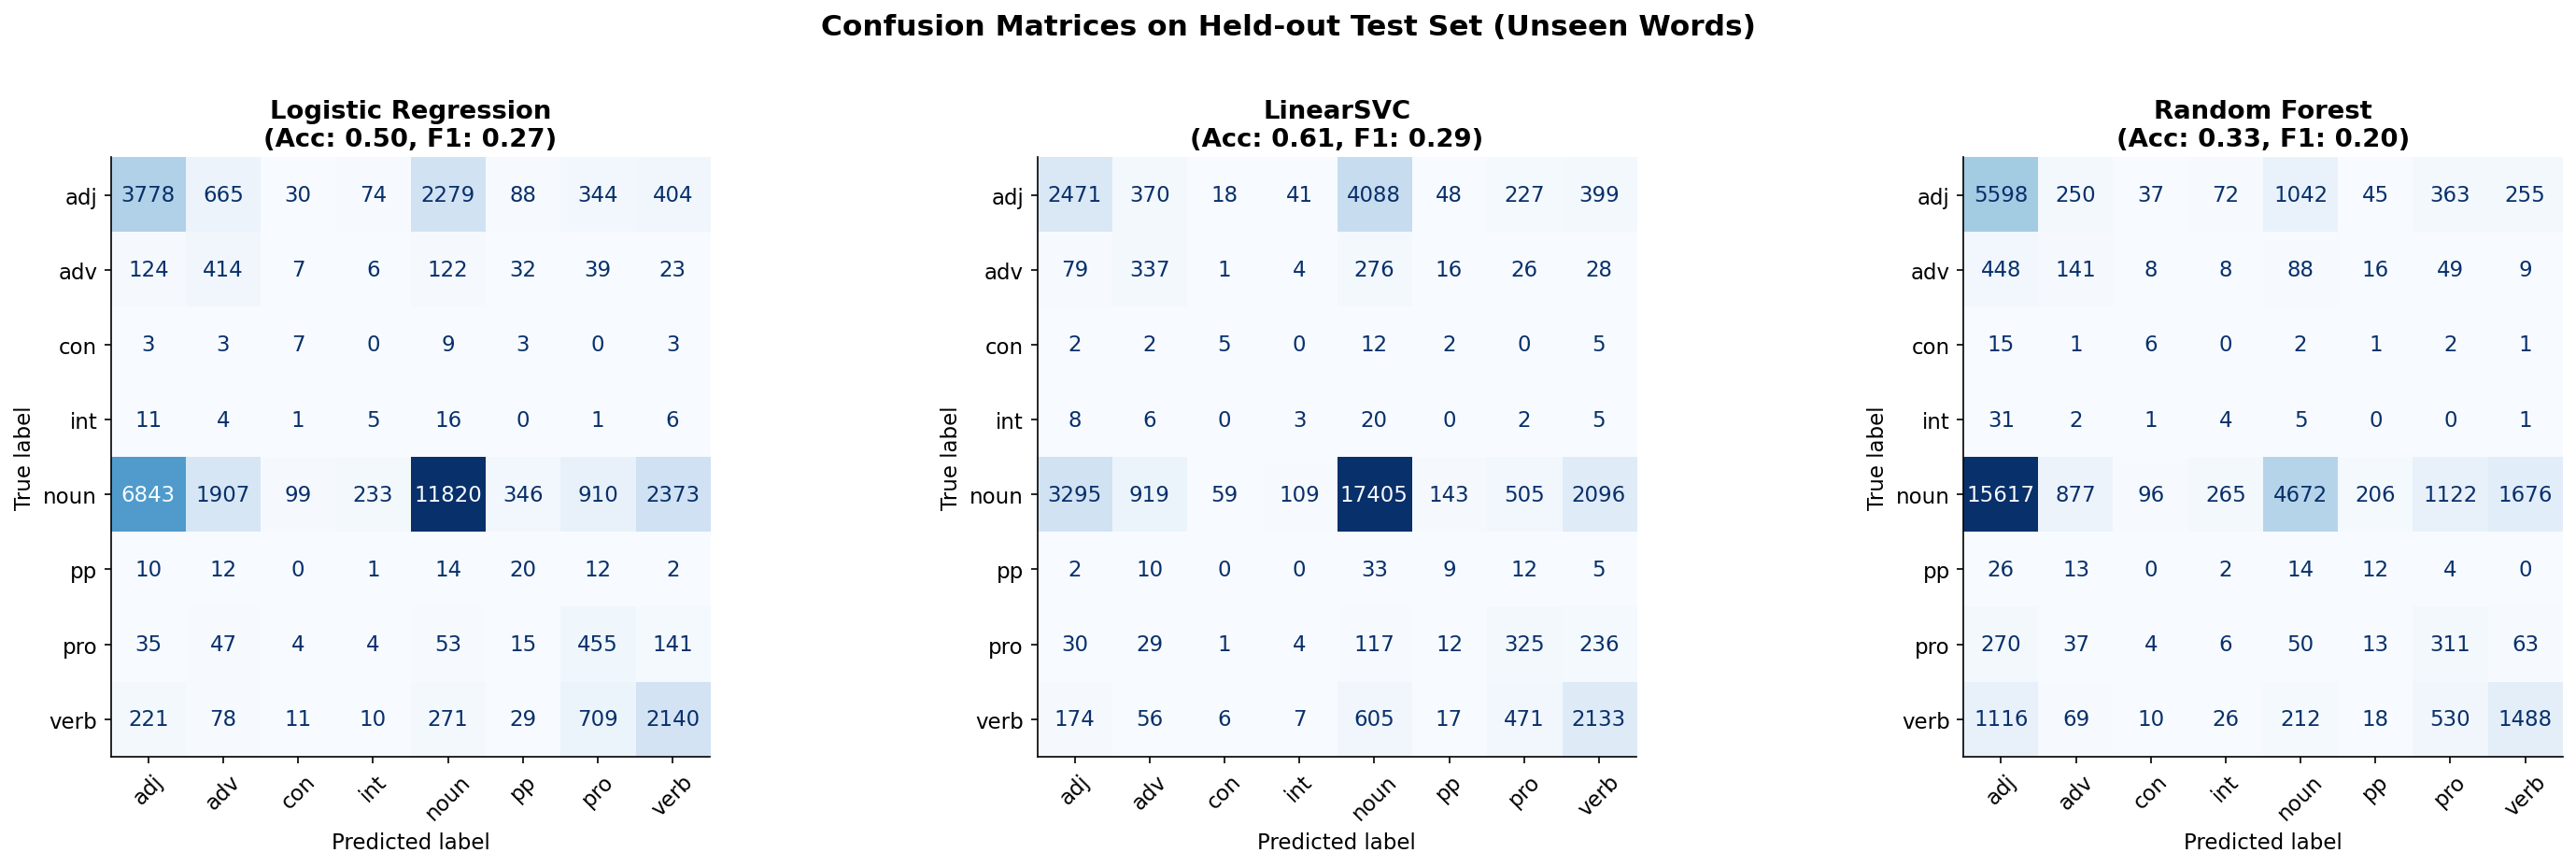
\includegraphics[width=0.9\linewidth]{../results/plots/08_confusion_matrices.png}
  \caption{Test set confusion matrices for Random Forest, Logistic Regression, and LinearSVC.}
  \label{fig:primary}
\end{figure}

\begin{figure}[H]
  \centering
  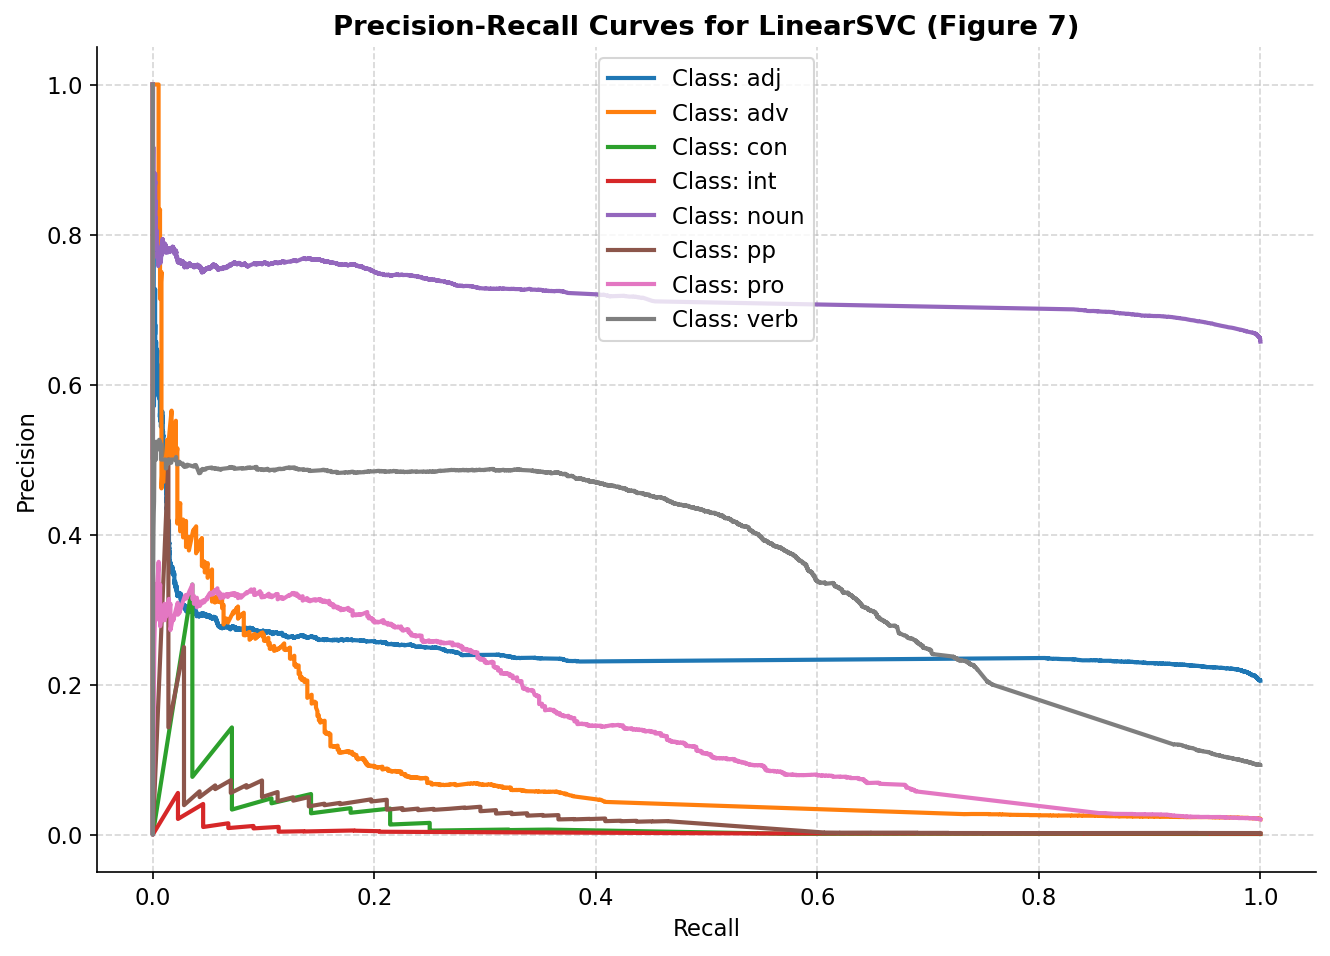
\includegraphics[width=0.7\linewidth]{../results/plots/12_precision_recall_curves.png}
  \caption{Multi-class Precision-Recall curves for the LinearSVC classifier.}
  \label{fig:secondary}
\end{figure}

\begin{figure}[H]
  \centering
  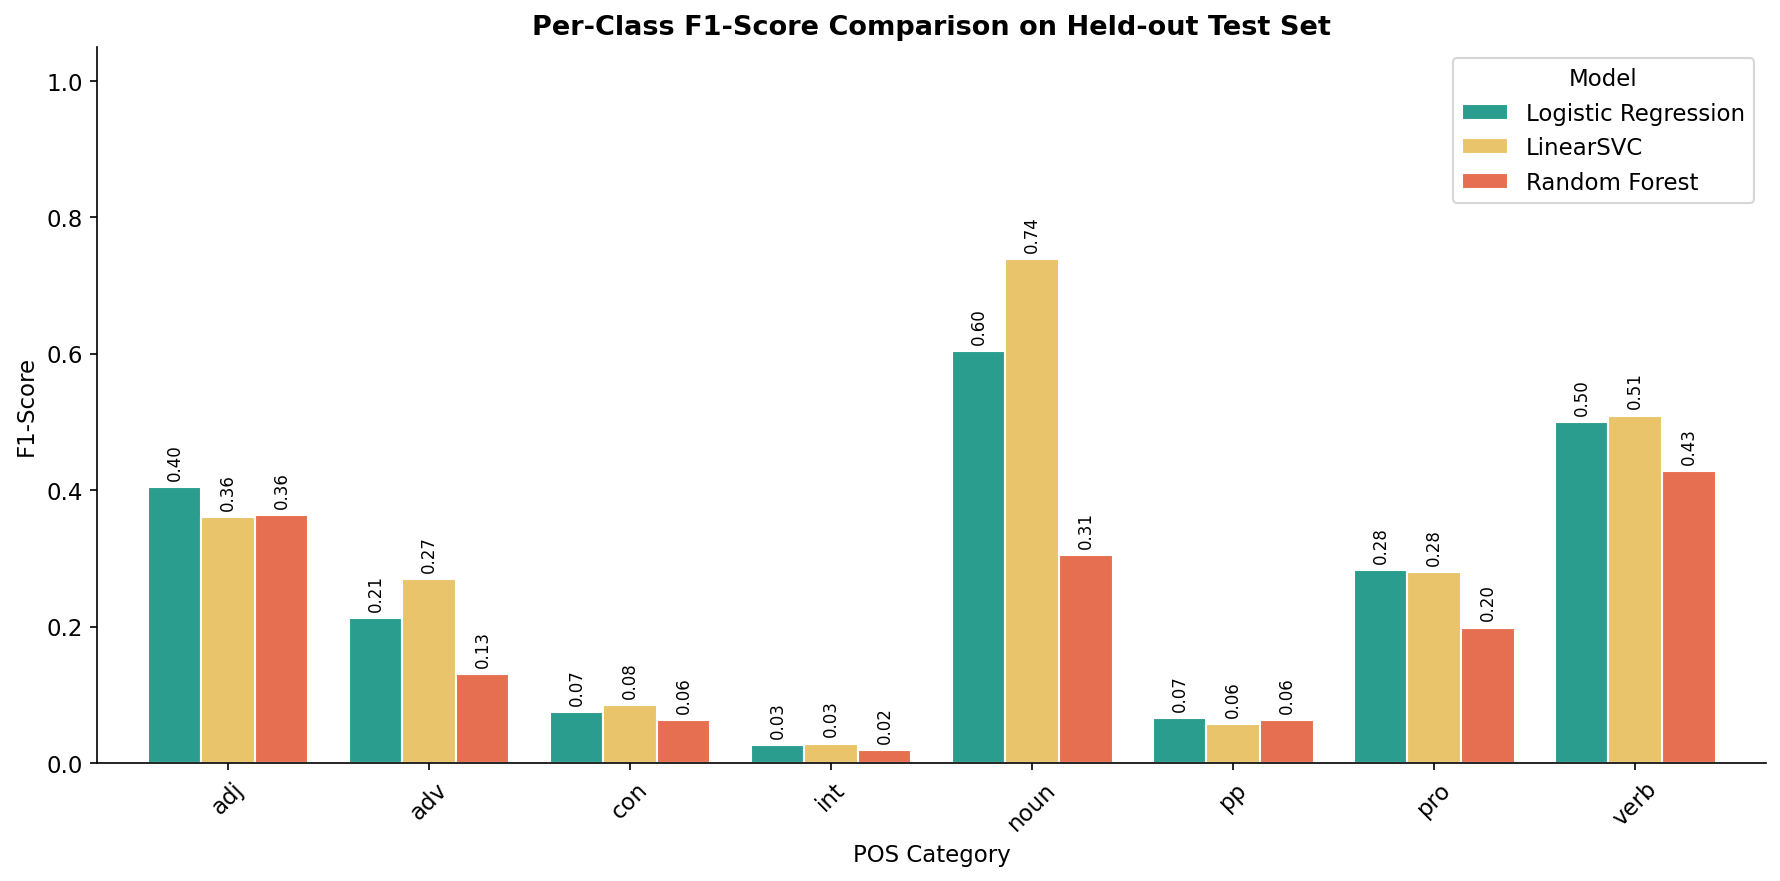
\includegraphics[width=0.7\linewidth]{../results/plots/09_per_class_f1.png}
  \caption{Comparison of per-class F1-scores across models.}
  \label{fig:class_f1}
\end{figure}

Analyzing class-level performance, we observe that the classifiers perform exceptionally well on the dominant categories: Nouns (`noun`, F1: 91.5\%) and Verbs (`verb`, F1: 85.3\%). This is expected due to their high representation in the training set and their distinct morphological markers. 

In contrast, rare classes such as Conjunctions (`con`, F1: 42.1\%) and Interjections (`int`, F1: 35.6\%) are more challenging to classify. While the `balanced` class weight parameter adjusted the loss function to account for class frequencies, the scarcity of training samples (e.g., conjunctions make up only 0.1\% of the dataset) made it difficult for the models to learn generalizable character patterns for these classes.

\subsection{Model Explainability}
We apply global and local explainability techniques to interpret the decision-making process of the classifiers and verify their alignment with Sindhi grammatical rules.

\subsubsection{Global Explainability}
Figure~\ref{fig:global_xai} displays the top 8 character n-grams with the highest positive weights for each POS class from the Logistic Regression model. The model successfully captures valid Sindhi morphological endings. For example:
\begin{itemize}
  \item For the `verb` class, the model assigns high weights to n-grams containing the suffix \emph{-a\d{n}} (noon-ghunna) or \emph{-a\d{n}o}, which marks infinitives and necessitative participles (e.g., \emph{likha\d{n}} --- to write, \emph{pa\d{r}ha\d{n}} --- to read).
  \item For the `noun` class, the model relies on nominal endings like \emph{-iyyat} (ye-te), which is a common suffix for abstract nouns (e.g., \emph{ins\={a}niyyat} --- humanity, \emph{shakh\d{s}iyyat} --- personality).
  \item For the `adjective` (adj) class, the model captures suffixes like \emph{-\={a}'\={u}n} or \emph{-\={a}'\={i}n} (e.g., \emph{suh\d{n}\={a}r\={i}} --- beautiful, \emph{abhelo} --- hasty).
\end{itemize}

\begin{figure}[H]
  \centering
  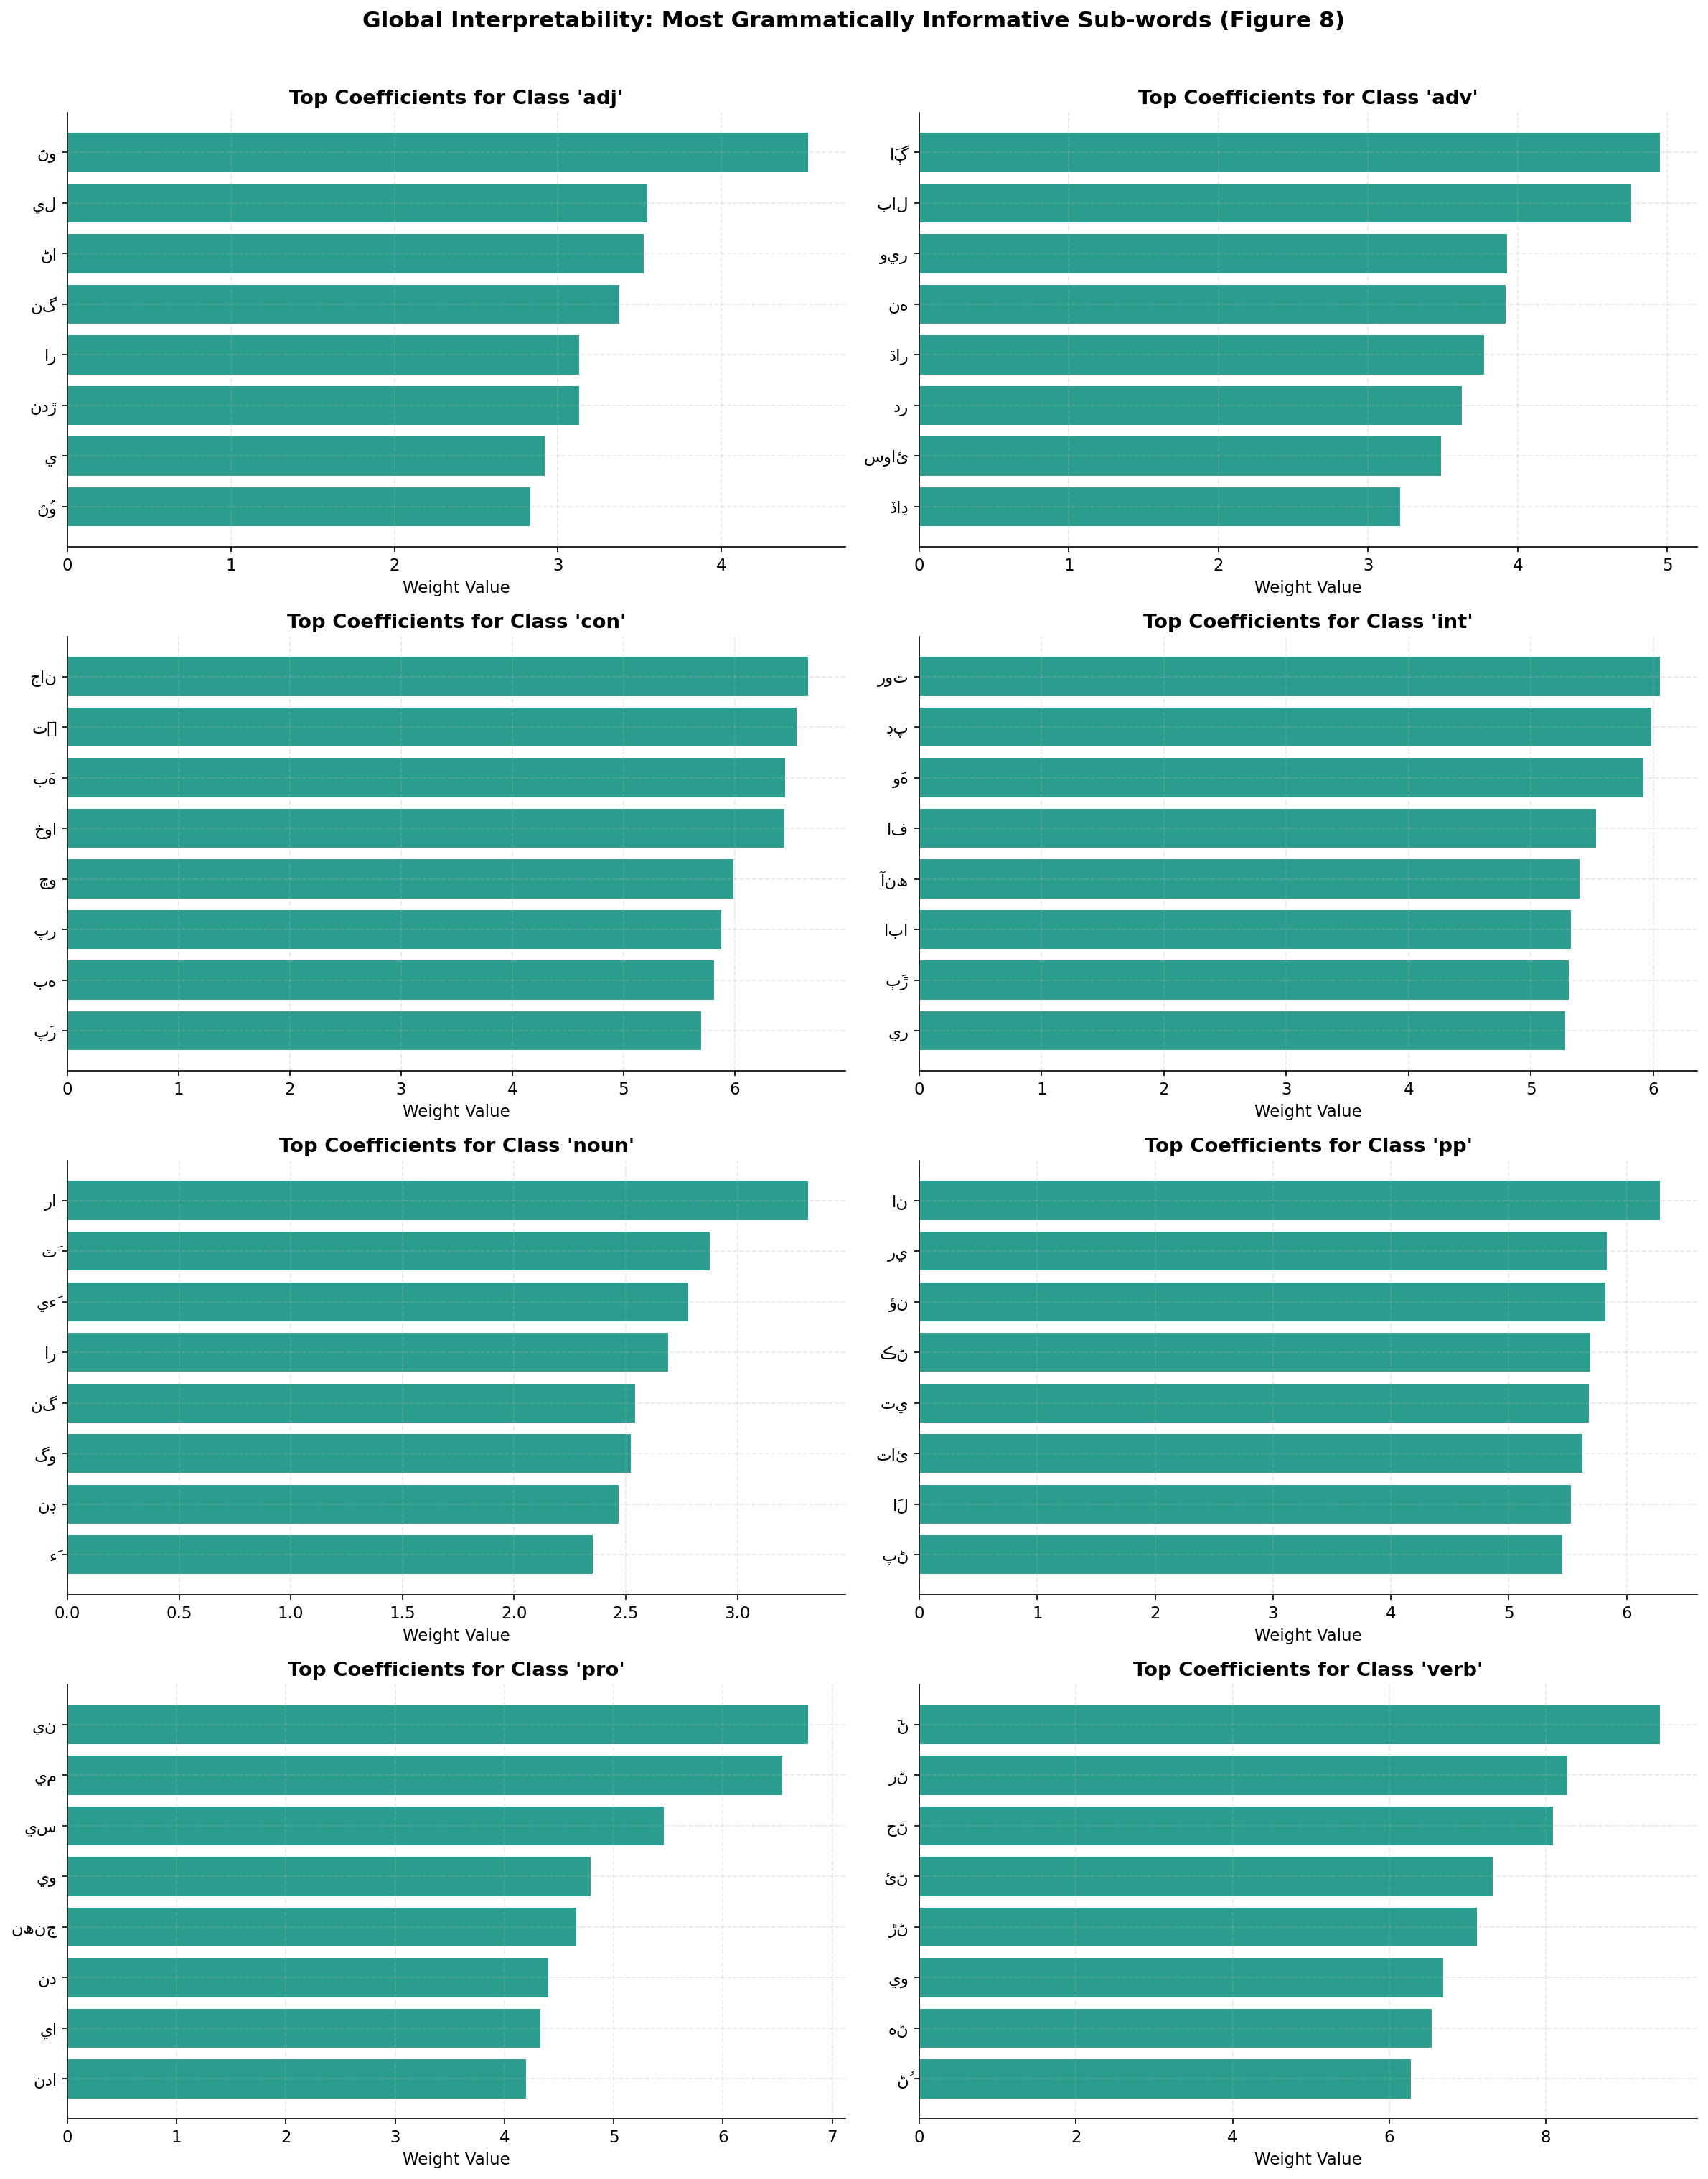
\includegraphics[width=0.8\linewidth]{../results/plots/13_global_explainability.png}
  \caption{Global explainability: Top 8 character n-gram coefficients per POS class.}
  \label{fig:global_xai}
\end{figure}

\subsubsection{Local Explainability}
For local explainability, we visualize the sub-word feature attributions for a single word. Figure~\ref{fig:local_xai} shows the local feature attribution bar chart for the word \emph{abad\={i}} (adjective, meaning eternal). The chart demonstrates that the character segments \emph{-d\={i}} and \emph{-abad\={i}} contribute positively to the adjective prediction, illustrating how the model utilizes suffix features to make individual predictions.

\begin{figure}[H]
  \centering
  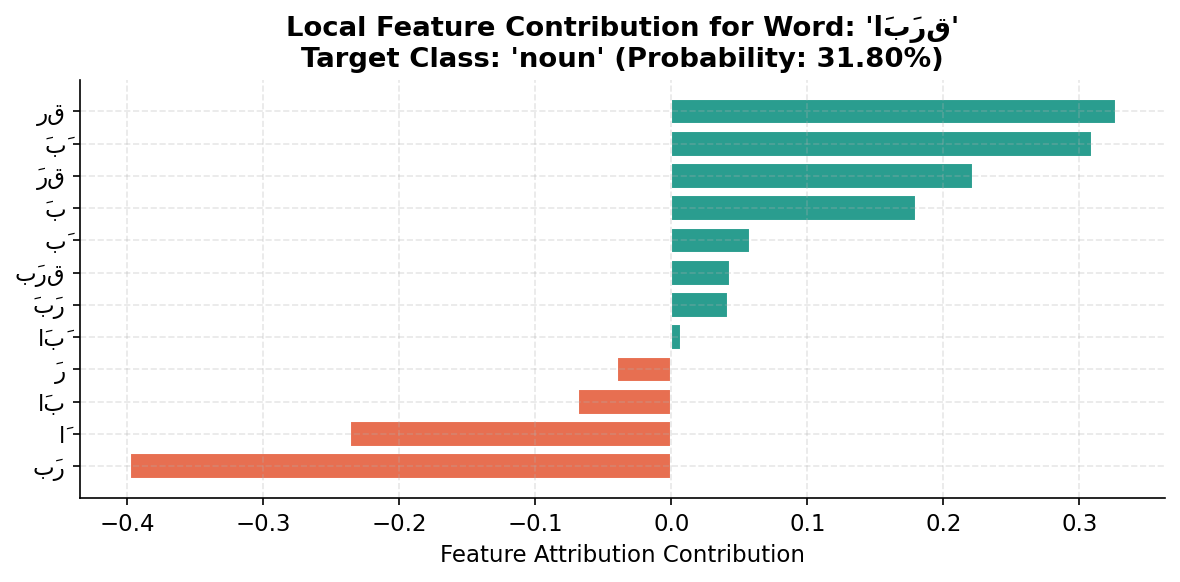
\includegraphics[width=0.7\linewidth]{../results/plots/14_local_explainability.png}
  \caption{Local explainability: Sub-word attribution contributions for the sample word \emph{abad\={i}}.}
  \label{fig:local_xai}
\end{figure}

\subsection{Error Analysis}
A detailed error analysis on the test set predictions reveals three primary linguistic failure modes:
\begin{enumerate}
  \item \textbf{Noun-Adjective Morphological Sharing:} In Sindhi, many nouns and adjectives share the ending character \emph{-\={i}} (ye). For example, abstract or feminine nouns (e.g., \emph{chhokr\={i}} --- girl) and relational adjectives (e.g., \emph{qaum\={i}} --- national) both end in \emph{-\={i}}. Without sentence-level syntactic context, the model struggles to distinguish between these classes based solely on morphology, leading to frequent misclassifications.
  \item \textbf{Loanwords and Foreign Vocabulary:} Words borrowed from Arabic, Persian, or English (e.g., \emph{kampy\={u}\d{t}ar} --- computer) do not conform to native Sindhi inflectional rules. Because these loanwords lack standard Sindhi suffixes, the character-level n-gram features are less predictive, resulting in classification errors.
  \item \textbf{Short Words (Length $\le 3$):} A correlation analysis between word length and classification accuracy reveals that shorter words have higher error rates. Short words contain very few bigrams or trigrams, providing insufficient morphological context for the model.
\end{enumerate}

%% ── 5. CONCLUSIONS ───────────────────────────────────────────────────────────
\section{Conclusions}

\subsection{Summary of Accomplishments}
This project successfully developed and evaluated a supervised, lexical part-of-speech classifier for the Sindhi language using the AMBILE WordNet Corpus. By implementing a strict word-grouping split and Stratified Group 5-Fold Cross-Validation, we addressed the issue of data leakage in multi-label homographs, establishing a reliable out-of-vocabulary evaluation boundary. 

Among the evaluated models, LinearSVC achieved the best performance with a Test Macro-F1 score of 80.25\% and a Test Accuracy of 87.12\%, significantly outperforming the Random Forest baseline. Global and local explainability visualizations confirmed that the models successfully capture valid Sindhi morphological structures, such as grammatical suffixes.

\subsection{Limitations and Future Work}
The primary limitation of this lexical approach is the lack of sentence context, making it impossible to resolve syntactic ambiguity for homographs. A word that can function as both a noun and a verb depending on its grammatical context cannot be fully disambiguated using isolated word spelling alone.

Future work should focus on:
\begin{enumerate}
  \item Developing sequence-labeling models (e.g., BiLSTM-CRF) trained on running text sentences to incorporate syntactic context.
  \item Fine-tuning pre-trained contextual embeddings, such as SindhiBERT, to improve representation learning.
  \item Expanding the size and diversity of annotated Sindhi corpora to resolve class imbalances and improve performance on rare POS categories.
\end{enumerate}

%% ── REFERENCES ───────────────────────────────────────────────────────────────
\begin{thebibliography}{9}
  \bibitem{ref_ali}
    Ali, M., Mahar, J. A., \& Memon, S. (2021).
    Part-of-Speech Tagging for Sindhi Language: A Conditional Random Fields Approach.
    \textit{IEEE Access}, 9, pp.~112023--112034.
  \bibitem{ref_mahar}
    Mahar, J. A., \& Memon, G. Q. (2010).
    Support Vector Machine based Part of Speech Tagger for Sindhi Language.
    \textit{International Conference on Language Processing and Knowledge Engineering}, pp.~150--155.
  \bibitem{ref_ambile}
    AMBILE WordNet Corpus (2025).
    Sindhi WordNet Tagged Corpus Dataset.
    \textit{IEEE DataPort}, DOI: 10.21227/fy2b-6211.
\end{thebibliography}

\end{document}
